\definecolor{dkgreen}{rgb}{0,0.6,0}
\definecolor{gray}{rgb}{0.5,0.5,0.5}
\definecolor{mauve}{rgb}{0.58,0,0.82}
\lstset{frame=tb,
	language=Java,
	aboveskip=3mm,
	belowskip=3mm,
	showstringspaces=false,
	columns=flexible,
	basicstyle=\rmfamily\fontsize{10.5pt}{12.6pt}\selectfont,
	numbers=none,
	numberstyle=\tiny\color{gray},
	keywordstyle=\color{blue},
	commentstyle=\color{dkgreen},
	stringstyle=\color{mauve},
	breaklines=true,
	breakatwhitespace=true,
	tabsize=3
}
\chapter{System Design} \label{chap:system-design}

\section{Design Overview}
In this section, the overview design of the system is described.

\subsection{Architecture Design}

This is the Architecture Design.

\begin{figure}[!h]
	\centering
	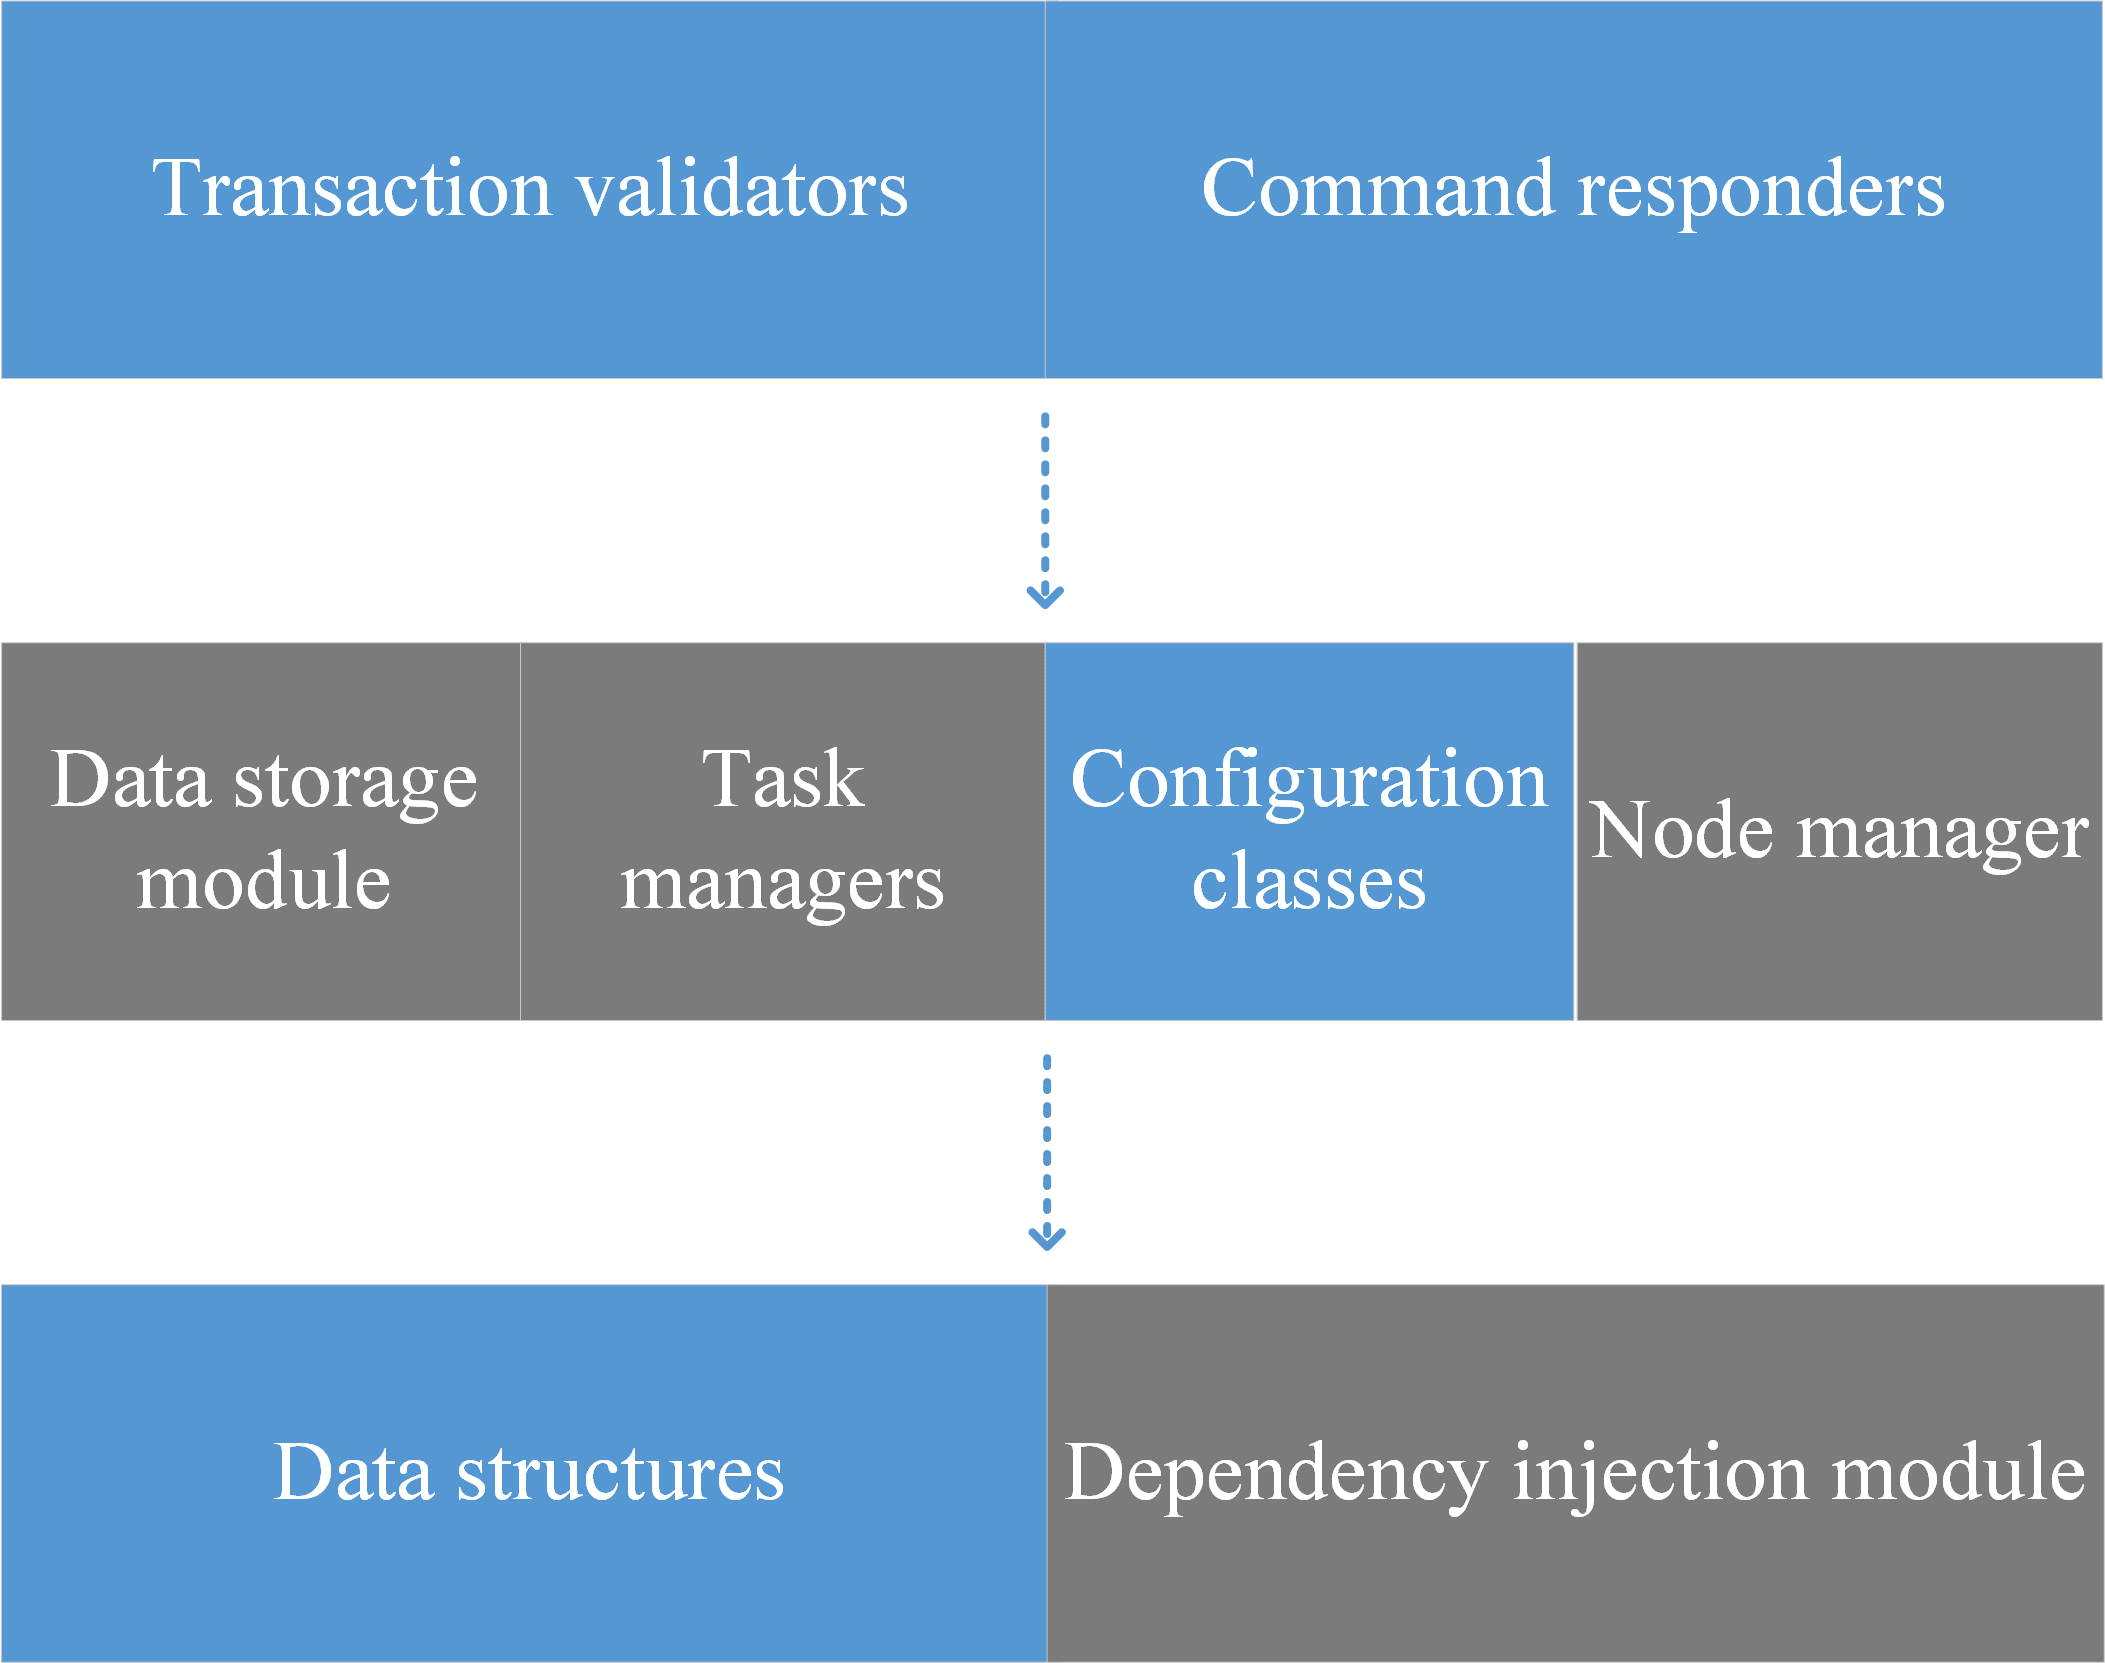
\includegraphics[width=0.65\textwidth]{Architecture_Sketch_Map}
	\caption{Architecture sketch map}
	\label{fig:architecture-sketch-map}
\end{figure}

\subsection{Module Design}

This is the Module Design.

\begin{figure}[!htbp]
	\centering
	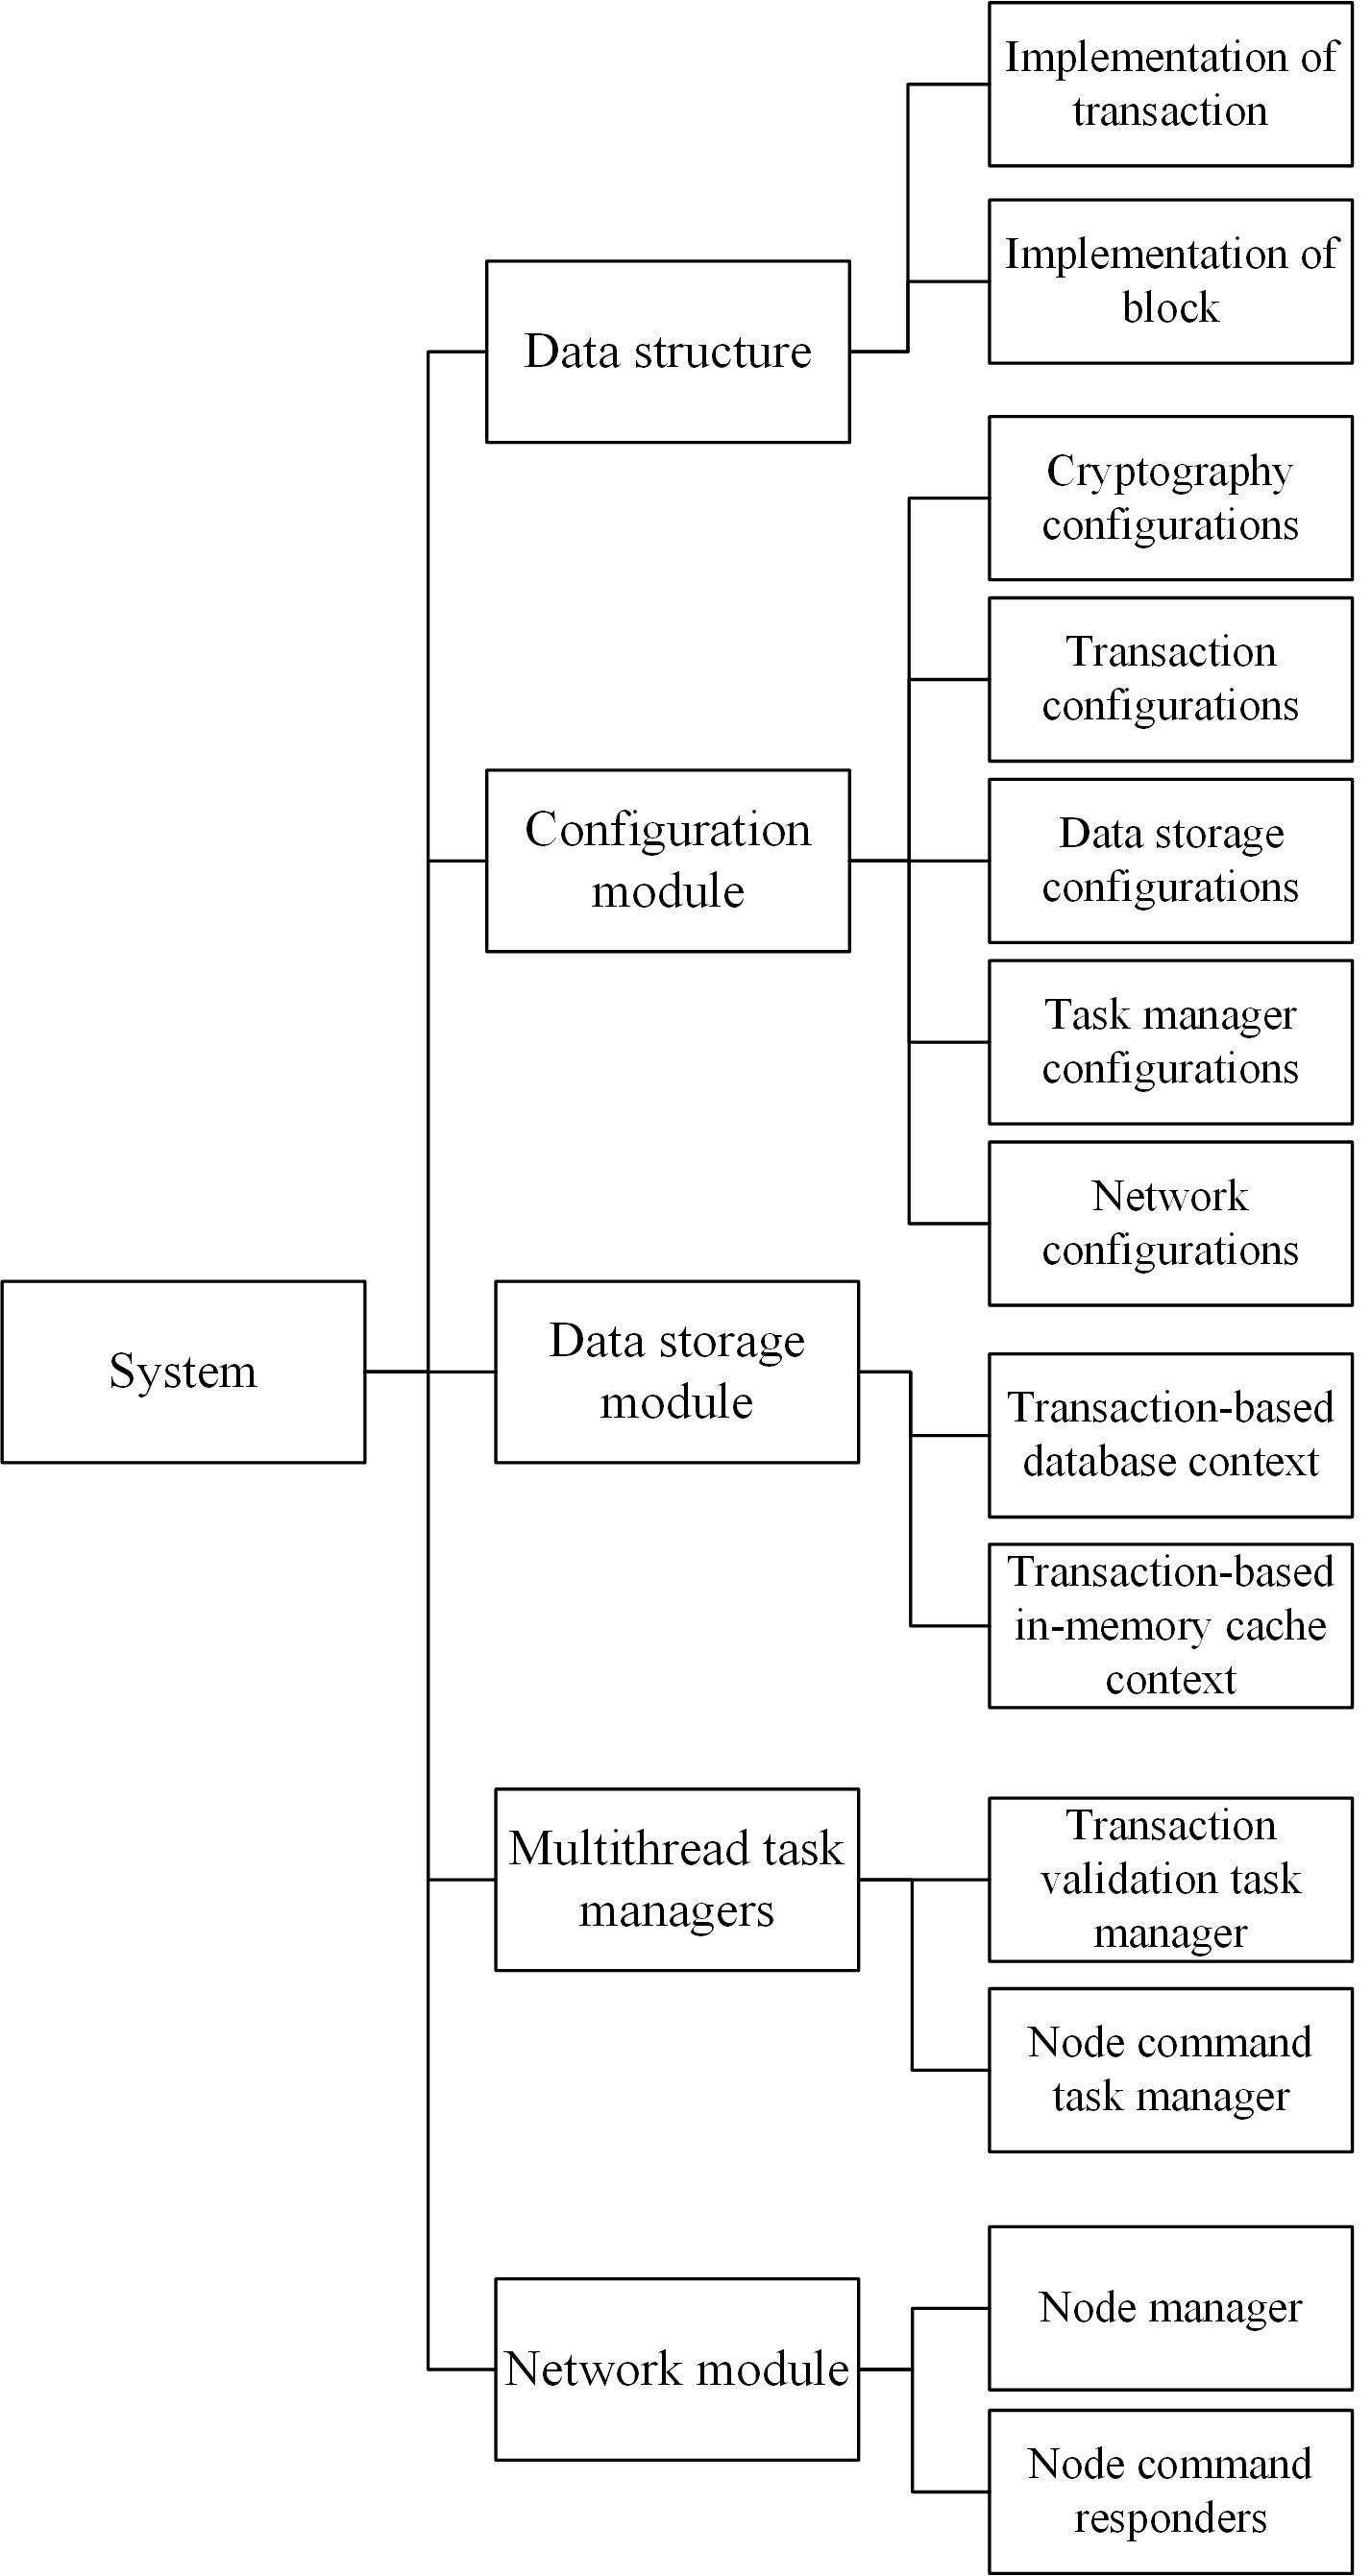
\includegraphics[max width=0.6\textwidth]{Module_Design_(Integrated,_Modules_Evenly_Distributed)}
	\caption{Module design sketch map}
	\label{fig:module-design}
\end{figure}

% \section{Detailed Design}\label{sec:system-design:detailed-design}
% In this section, the detailed design of the system is presented, following the order of module division mentioned above.

\subsection{Data Structure}

\begin{table}[!htbp]
\setlength{\abovecaptionskip}{0cm}%  
\setlength{\belowcaptionskip}{-0.1cm}%设置表名与表间距离
\centering
\caption{Data structure of a block in Bitcoin}
\label{tab:block_in_bitcoin}
 
\begin{small}
	\begin{tabular}{l l}
		\Xhline{1.5pt}
		{\bfseries Field} & {\bfseries Purpose} \\
		\Xhline{1.5pt}
		version & Version of the block \\
		\hline
		hashPrevBlock & Hash of the previous block \\
		\hline
		hashMerkleRoot & Hash of Merkle root; for indexing transactions and ensuring validity of them \\
		\hline
		time & Unix epoch in UTC \\
		\hline
		bits & Contains info about the hash target of PoW or interpreted as the difficulty \\
		\hline
		nonce & A random number; involved in hash generation of the block \\
		\hline
		transactions & Transactions included in the block \\
		\Xhline{1.5pt}
	\end{tabular}
\end{small}
\end{table}

\section{Summary}
This chapter demonstrates the overall architecture and more detailed designs including the data structures, several modules and the general startup procedures. Some contents have been described as to what design pattern can be used and how extensions can be built using the interfaces. They will guide the implementations in the next chapter.

